% Options for packages loaded elsewhere
\PassOptionsToPackage{unicode}{hyperref}
\PassOptionsToPackage{hyphens}{url}
%
\documentclass[
]{article}
\usepackage{amsmath,amssymb}
\usepackage{lmodern}
\usepackage{iftex}
\ifPDFTeX
  \usepackage[T1]{fontenc}
  \usepackage[utf8]{inputenc}
  \usepackage{textcomp} % provide euro and other symbols
\else % if luatex or xetex
  \usepackage{unicode-math}
  \defaultfontfeatures{Scale=MatchLowercase}
  \defaultfontfeatures[\rmfamily]{Ligatures=TeX,Scale=1}
\fi
% Use upquote if available, for straight quotes in verbatim environments
\IfFileExists{upquote.sty}{\usepackage{upquote}}{}
\IfFileExists{microtype.sty}{% use microtype if available
  \usepackage[]{microtype}
  \UseMicrotypeSet[protrusion]{basicmath} % disable protrusion for tt fonts
}{}
\makeatletter
\@ifundefined{KOMAClassName}{% if non-KOMA class
  \IfFileExists{parskip.sty}{%
    \usepackage{parskip}
  }{% else
    \setlength{\parindent}{0pt}
    \setlength{\parskip}{6pt plus 2pt minus 1pt}}
}{% if KOMA class
  \KOMAoptions{parskip=half}}
\makeatother
\usepackage{xcolor}
\IfFileExists{xurl.sty}{\usepackage{xurl}}{} % add URL line breaks if available
\IfFileExists{bookmark.sty}{\usepackage{bookmark}}{\usepackage{hyperref}}
\hypersetup{
  pdftitle={Trabalho final - IAED 2021},
  pdfauthor={Matheus Willian Polato - RA 181024462},
  pdflang={pt-br},
  hidelinks,
  pdfcreator={LaTeX via pandoc}}
\urlstyle{same} % disable monospaced font for URLs
\usepackage[margin=1in]{geometry}
\usepackage{graphicx}
\makeatletter
\def\maxwidth{\ifdim\Gin@nat@width>\linewidth\linewidth\else\Gin@nat@width\fi}
\def\maxheight{\ifdim\Gin@nat@height>\textheight\textheight\else\Gin@nat@height\fi}
\makeatother
% Scale images if necessary, so that they will not overflow the page
% margins by default, and it is still possible to overwrite the defaults
% using explicit options in \includegraphics[width, height, ...]{}
\setkeys{Gin}{width=\maxwidth,height=\maxheight,keepaspectratio}
% Set default figure placement to htbp
\makeatletter
\def\fps@figure{htbp}
\makeatother
\setlength{\emergencystretch}{3em} % prevent overfull lines
\providecommand{\tightlist}{%
  \setlength{\itemsep}{0pt}\setlength{\parskip}{0pt}}
\setcounter{secnumdepth}{-\maxdimen} % remove section numbering
\ifLuaTeX
\usepackage[bidi=basic]{babel}
\else
\usepackage[bidi=default]{babel}
\fi
\babelprovide[main,import]{brazilian}
% get rid of language-specific shorthands (see #6817):
\let\LanguageShortHands\languageshorthands
\def\languageshorthands#1{}
\ifLuaTeX
  \usepackage{selnolig}  % disable illegal ligatures
\fi

\title{Trabalho final - IAED 2021}
\author{Matheus Willian Polato - RA 181024462}
\date{2021/2022}

\begin{document}
\maketitle

\hypertarget{introduuxe7uxe3o}{%
\section{Introdução}\label{introduuxe7uxe3o}}

Este documento refere-se ao trabalho final da disciplina de Introdução à
Análise Exploratória de Dados, ministrada pelo professor João Pedro
Albino, no ano de 2021/2022, pela Faculdade de Ciências - UNESP Câmpus
de Bauru. O projeto consiste em realizar uma Análise Exploratória de
Dados em relação a pandemia causada pelo Coronavírus (COVID-19) e como
está impactando a vida das pessoas na cidade de Bauru. As análises
realizadas mostram a distribuição de mortes de acordo com a idade dos
pacientes, gênero, quais as características das comorbidades dos óbitos,
a variação periódica de tais óbitos, tipos e tempo de permanência
hospitalar dos pacientes e a relação entre óbitos ocorridos e a
vacinação dos falecidos.

\hypertarget{anuxe1lise-exploratuxf3ria-dos-dados}{%
\section{Análise Exploratória dos
Dados}\label{anuxe1lise-exploratuxf3ria-dos-dados}}

\hypertarget{uxf3bitos-entre-guxeaneros}{%
\subsection{Óbitos entre gêneros}\label{uxf3bitos-entre-guxeaneros}}

Foi realizada uma análise para verificar qual a taxa de óbitos entre os
gêneros. O gráfico a seguir mostra o que foi obtido.

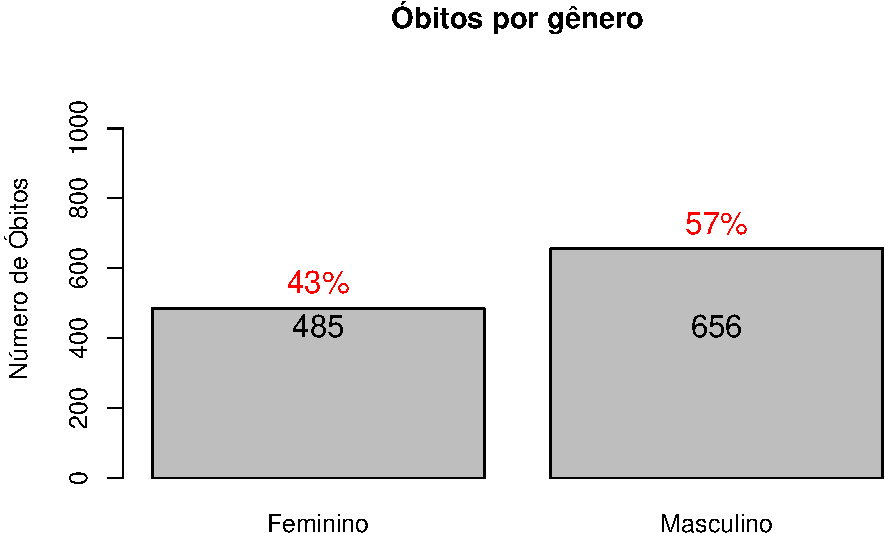
\includegraphics{tf-matheus-willian_files/figure-latex/unnamed-chunk-1-1.pdf}

Pode-se verificar que a maior parte dos óbitos são do gênero masculino,
com 57\%, seguido do gênero feminino, com 43\%.

\hypertarget{distribuiuxe7uxe3o-dos-uxf3bitos-de-acordo-com-a-idade-dos-pacientes}{%
\subsection{Distribuição dos óbitos de acordo com a idade dos
pacientes}\label{distribuiuxe7uxe3o-dos-uxf3bitos-de-acordo-com-a-idade-dos-pacientes}}

Foi realizado uma análise para verificar qual a distribuição dos óbitos
de acordo com a idade dos pacientes.
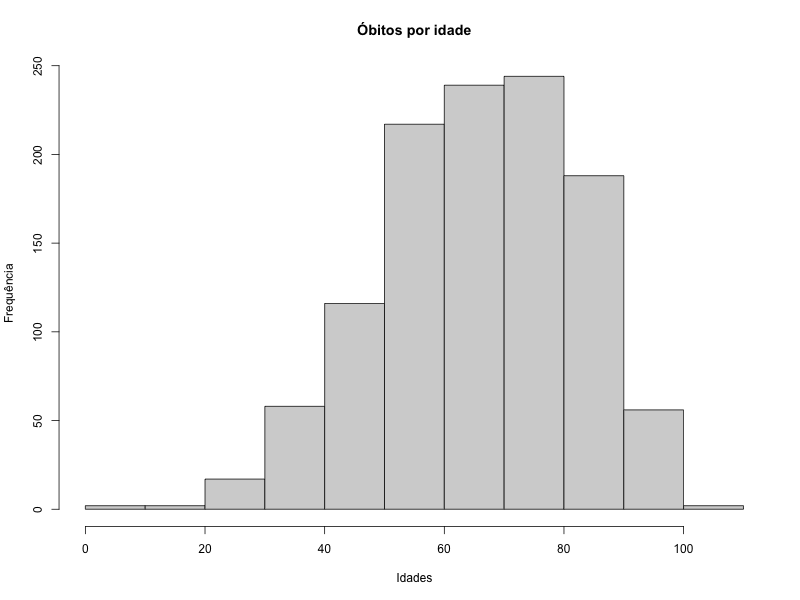
\includegraphics{../graficos/histograma_obitos_por_idade.png}

Pode-se constatar no histograma que a maior frequência de mortes está
concentrada entre as idades de 50 a 90 anos, seguida pela idade de 40 a
50. Isso mostra que o coronavírus tem mais impacto em pessoas com idades
mais avançadas.

\hypertarget{caracteruxedsticas-das-principais-comorbidades-dos-uxf3bitos}{%
\subsection{Características das principais comorbidades dos
óbitos}\label{caracteruxedsticas-das-principais-comorbidades-dos-uxf3bitos}}

Foi realizado uma análise para verificar quais as características das
principais comorbidades dos óbitos. A tabela e o gráfico a seguir
mostram quais as comorbidades que mais sofreram óbitos.

\begin{verbatim}
##                Comorbidades Freq
## 140             hipertensão   80
## 15              cardiopatia   69
## 50                 diabetes   61
## 86   diabetes e hipertensão   55
## 183               obesidade   50
## 166 hipertensão e obesidade   41
\end{verbatim}

\begin{figure}
\centering
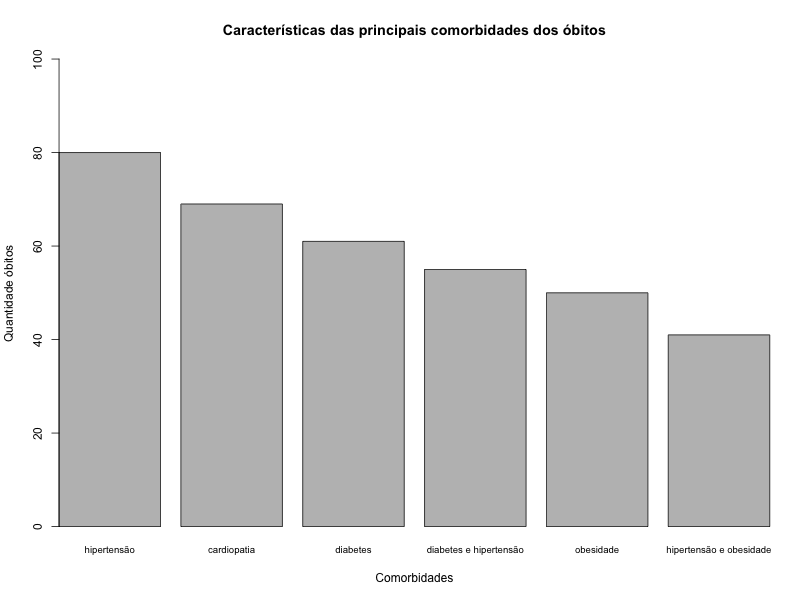
\includegraphics{../graficos/caracteristicas_principais_comorbidades_obitos.png}
\caption{Características das principais comorbidades dos óbitos}
\end{figure}

Pode-se constatar que hipertensão é a comorbidade mais atingida pelo
coronavírus, com um total de 80 óbitos. É possível verificar também que
a hipertensão, em conjunto com outra comorbidade, também está entre as 6
comorbidades mais atingidas. Ocorreram 55 óbitos de pessoas que possuíam
diabetes e hipertensão e 41 óbitos de pessoas que possuíam hipertensão e
obesidade.

\hypertarget{variauxe7uxe3o-periuxf3dica-dos-uxf3bitos}{%
\subsection{Variação periódica dos
óbitos}\label{variauxe7uxe3o-periuxf3dica-dos-uxf3bitos}}

Foi realizado uma análise para verificar a variação periódica dos
óbitos. O gráfico mostra o que foi obtido.

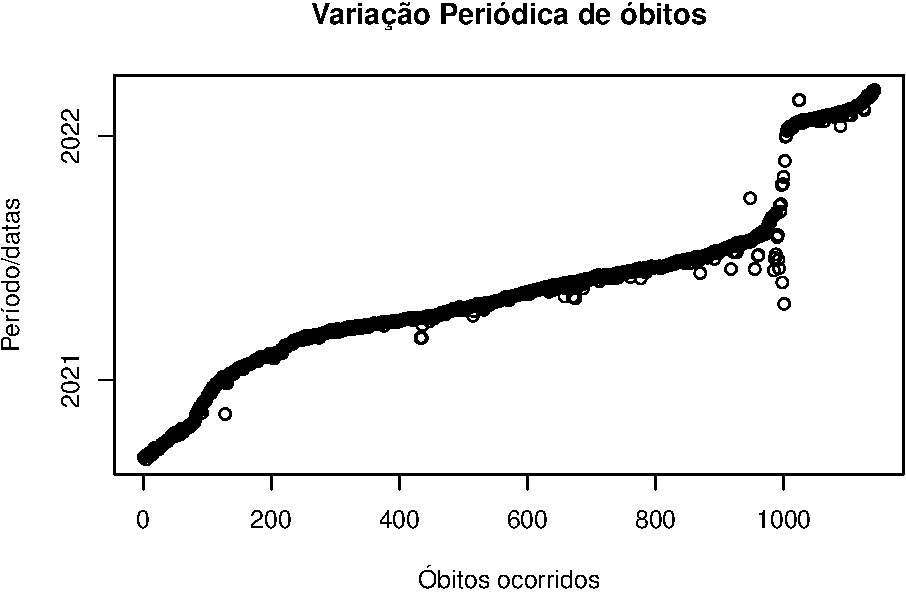
\includegraphics{tf-matheus-willian_files/figure-latex/unnamed-chunk-3-1.pdf}

É possível perceber que os óbitos não ficaram estáveis em nenhum
momento, a linha está em uma constante crescente, porém menos que no
período antes de 2021. Isso mostra que a vacinação é sim eficaz, mas
ainda é necessário uma atenção por parte da população, para cada um
fazer sua parte, utilizar máscara e evitar aglomerações.

\hypertarget{tipos-e-tempo-de-permanuxeancia-hospitalar}{%
\subsection{Tipos e tempo de permanência
hospitalar}\label{tipos-e-tempo-de-permanuxeancia-hospitalar}}

\hypertarget{tipo-de-permanuxeancia-hospitalar}{%
\subsubsection{Tipo de permanência
hospitalar}\label{tipo-de-permanuxeancia-hospitalar}}

Foi realizado uma análise para verificar a quantidade de cada tipo de
hospitalização. A tabela a seguir mostra os dados obtidos.

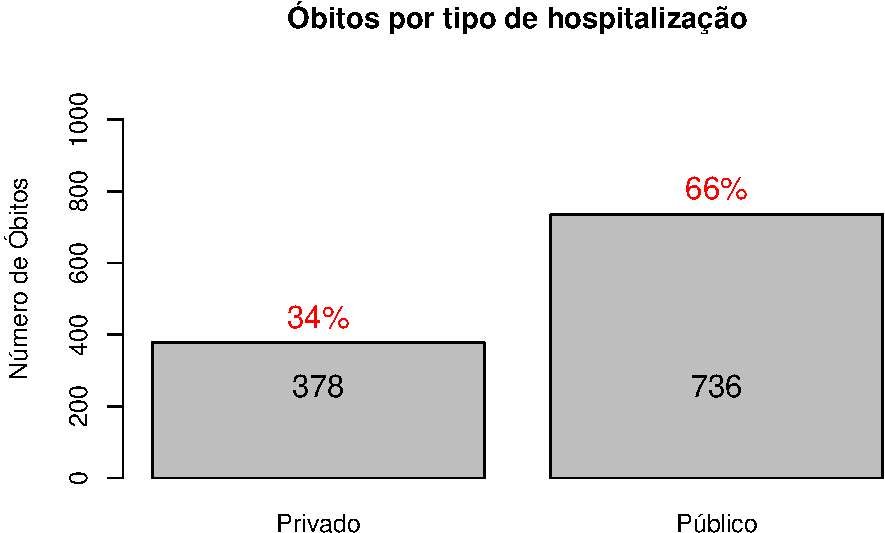
\includegraphics{tf-matheus-willian_files/figure-latex/unnamed-chunk-4-1.pdf}

Percebe-se que a maioria das hospitalizações foram em hospitais
públicos, o que explica o rápido esgotamento de leitos nas unidades
públicas de saúde.

\hypertarget{tempo-de-permanuxeancia-hospitalar}{%
\subsubsection{Tempo de permanência
hospitalar}\label{tempo-de-permanuxeancia-hospitalar}}

O próximo gráfico mostra o tempo de permanência hospitalar até o óbito.

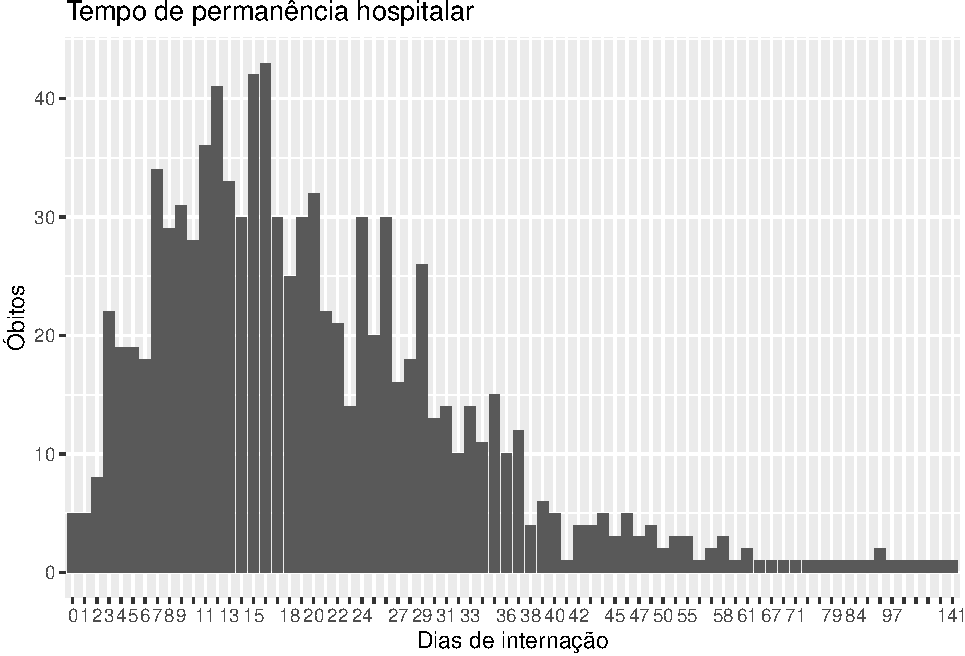
\includegraphics{tf-matheus-willian_files/figure-latex/unnamed-chunk-5-1.pdf}

É possível perceber que a maior parte dos pacientes que vieram a óbito
ficaram internados aproximadamente entre 3 e 36 dias.

\hypertarget{relauxe7uxe3o-entre-uxf3bitos-ocorridos-e-a-vacinauxe7uxe3o-dos-falecidos}{%
\subsection{Relação entre óbitos ocorridos e a vacinação dos
falecidos}\label{relauxe7uxe3o-entre-uxf3bitos-ocorridos-e-a-vacinauxe7uxe3o-dos-falecidos}}

Foi realizado uma análise para verificar a relação entre os óbitos e a
vacinação dos falecidos. A tabela a seguir mostra os dados obtidos.

\begin{verbatim}
##   Doses Freq
## 1     0 1020
## 2     1    5
## 3     2   66
## 4     3   51
\end{verbatim}

Pode-se constatar que a maior frequência de óbitos foram das pessoas que
ainda não haviam tomado nenhuma dose da vacina, com um total de 1020
pessoas. A segunda maior frequência é de pessoas que tomaram 2 doses,
com um total de 66. Pessoas que tomaram apenas uma dose da vacina têm um
total de 5. Uma observação para isso é que, entre essas pessoas, pode
conter aquelas que tomaram a dose única, ou seja, estavam totalmente
imunizadas.

\hypertarget{conclusuxe3o}{%
\section{Conclusão}\label{conclusuxe3o}}

Com este trabalho foi possível analisar alguns dados referentes aos
óbitos por conta da COVID-19 na cidade de Bauru. Pode-se concluir que o
vírus afetou muita gente, não somente bauruenses. É necessário continuar
seguindo os protocolos de segurança, principalmente as pessoas que
possuem algum tipo de comorbidade. Também é necessário se vacinar, pois
como mostram as análises, o maior índice de óbitos são daqueles que não
se vacinaram.

\end{document}
